\chapter{Visualizing and Understanding CNNs}
\label{ch:lesson39}

A trained CNN is a black box because its millions of weights don't have obvious individual meanings. But \emph{where in the input image} a prediction comes from is answerable, and answering it is often what separates ``the model got the right answer'' from ``the model got the right answer for the right reason.'' This chapter builds two visualization tools from scratch --- \textbf{saliency maps} (\citelink{simonyan2013saliency}{Simonyan et al., 2014}) and \textbf{Grad-CAM} (\citelink{selvaraju2017}{Selvaraju et al., 2017}) --- on real photos from CIFAR-10 (\citelink{krizhevsky2009cifar}{Krizhevsky, 2009}), then uses them to catch a model that's cheating. Finally, \textbf{t-SNE} (\citelink{vandermaaten2008tsne}{Van der Maaten \& Hinton, 2008}) is used to visualize the learned feature vectors.

\section{Setup: a cat-vs-automobile CNN, with feature maps exposed}

A CIFAR-10 binary task: cat vs.\ automobile, 300 training images per class. The architecture is Chapter~\ref{ch:lesson34}'s CNN pattern, except \code{forward} now also returns the last convolutional layer's feature map (before global pooling), so both visualization methods have access to it. Trained for 300 epochs: test accuracy $86.5\%$.

\section{Saliency maps}

The idea of saliency maps (\citelink{simonyan2013saliency}{Simonyan et al., 2014}): take the gradient of the predicted class \emph{score} with respect to every input pixel. A pixel with a large-magnitude gradient is one where a small change would most change the prediction --- i.e., a pixel the network is ``looking at.''

\begin{lstlisting}
def saliency_map(model, img_hw3):
    x = torch.tensor(img_hw3).permute(2, 0, 1).unsqueeze(0)
    x.requires_grad_(True)
    score, feat = model(x)
    score.backward()
    return x.grad[0].abs().amax(dim=0).numpy(), feat  # max abs gradient across 3 color channels
\end{lstlisting}

\begin{figure}[h]
\centering
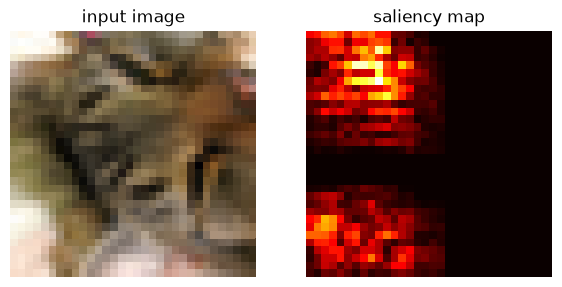
\includegraphics[width=0.55\textwidth]{figures/lesson39_fig01.png}
\caption{An input image and its saliency map --- brightest where the gradient of the class score with respect to that pixel is largest.}
\label{fig:l39-1}
\end{figure}

\section{Grad-CAM}

Raw saliency maps (Figure~\ref{fig:l39-1}) are pixel-level and tend to be noisy. \textbf{Grad-CAM} instead operates on the feature maps of a chosen convolutional layer, typically the last convolutional layer. Although these feature maps are lower-resolution than a pixel-level saliency map (downsampled by the pooling layers before them), they tend to carry more class-discriminative semantic information than individual raw-pixel gradients do. The method:
\begin{enumerate}
  \item Compute the gradient of the target class score with respect to each feature-map channel.
  \item Globally average each channel's gradients over its spatial dimensions to obtain one importance weight per channel.
  \item Take the weighted sum of the feature-map channels and apply ReLU, retaining the positive contributions to the target class.
\end{enumerate}
The resulting coarse heatmap has the spatial resolution of the selected convolutional layer; it can be upsampled to the input resolution for visualization (Figure~\ref{fig:l39-2}).

\begin{lstlisting}
def grad_cam(model, img_hw3, out_size=32):
    x = torch.tensor(img_hw3).permute(2, 0, 1).unsqueeze(0)
    x.requires_grad_(True)
    score, feat = model(x)
    feat.retain_grad()
    score.backward()
    weights = feat.grad[0].mean(dim=(1, 2))  # importance per channel
    cam = F.relu((weights[:, None, None] * feat[0]).sum(dim=0))
    return F.interpolate(cam[None, None], size=(out_size, out_size), mode='bilinear')[0, 0]
\end{lstlisting}

\begin{figure}[h]
\centering
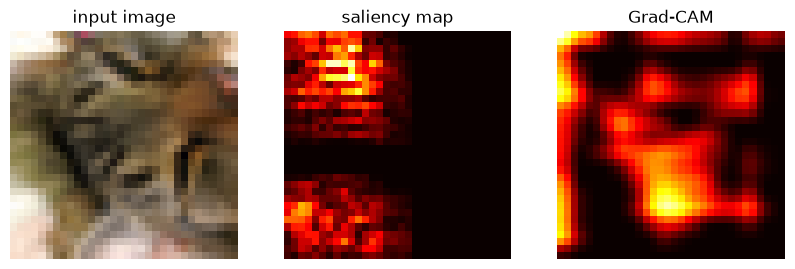
\includegraphics[width=0.85\textwidth]{figures/lesson39_fig02.png}
\caption{Input image, saliency map, and Grad-CAM heatmap, side by side.}
\label{fig:l39-2}
\end{figure}

\section{Do these maps actually track what the model uses?}

To test whether these tools are useful, deliberately give the model a shortcut, and check whether they correctly catch it. Add a small, unmistakable $5\times5$ white marker to the top-left corner of every \textbf{automobile} training image only (never on cat images) --- a stand-in for a real-world confound, like a watermark, a lab-specific artifact, or a capture-device quirk that happens to correlate with one class. Train a second model, \code{model\_shortcut}, on this corrupted dataset, and compare it against the original \code{model\_original} above (never exposed to any marker):

\begin{center}
\renewcommand{\arraystretch}{1.3}
\begin{tabular}{lrr}
\hline
 & \textbf{clean test} & \textbf{marked test} \\
\hline
model\_original & 86.5\% & 83.5\% \\
model\_shortcut & 63.0\% & 98.0\% \\
\hline
\end{tabular}
\end{center}

\code{model\_original}'s accuracy barely moves whether the marker is present or not --- since it never learned to use it, it has nothing to lose when it's absent. \code{model\_shortcut} looks \emph{better} than \code{model\_original} when the marker is present, but it collapses when the marker is removed. It learned the shortcut ``white corner square = automobile.''

Now use Grad-CAM to check whether the visualization tool actually catches this. Since the marker's location is known exactly (rows 0--4, columns 0--4), checking becomes: what fraction of test images does each model's heatmap peak land inside that exact $5\times5$ region?

\begin{center}
\renewcommand{\arraystretch}{1.3}
\begin{tabular}{llrr}
\hline
\textbf{model} & \textbf{test images} & \textbf{saliency} & \textbf{Grad-CAM} \\
\hline
model\_original & marked & 0.0\%   & 0.0\% \\
model\_shortcut & marked & 96.0\%  & 100.0\% \\
model\_shortcut & clean  & 56.0\%  & 92.0\% \\
\hline
\end{tabular}
\end{center}

\code{model\_original} (never trained on the marker) rarely lands either method's peak in that exact corner. \code{model\_shortcut} is a different story: on marked images both tools are nearly perfect (saliency 96\%, Grad-CAM 100\%), but on \emph{clean} images --- where the marker was never added, yet \code{model\_shortcut} still relies on it internally --- Grad-CAM's peak still lands there 92\% of the time versus only 56\% for saliency. Grad-CAM pools gradients over an entire feature-map channel before localizing, which smooths out pixel-level noise and makes it the more trustworthy detector when the shortcut's literal trigger isn't visible in a given image; \code{model\_shortcut}'s internal machinery is anchored to that spot regardless of what's actually there, exactly the failure mode described at the top of this chapter.

The practical lesson: accuracy alone (Chapter~\ref{ch:lesson36}) can't distinguish whether the model has learned the real signal or a shortcut correlated with it in the training data. Visualization tools such as saliency and Grad-CAM can --- but only if you know to check, if you pick a tool sturdy enough to trust, and if you interpret the results with some skepticism about what else in the image might be drawing gradient attention.

\section{Feature-space visualization: t-SNE}

Saliency maps and Grad-CAM both answer a \emph{spatial} question about one image at a time: where is the network looking? \textbf{t-SNE} (\citelink{vandermaaten2008tsne}{van der Maaten \& Hinton, 2008}) asks a broader question across many images: does the network's internal representation separate the classes it was trained to recognize? It takes each image's 16-d feature vector --- the representation fed directly to the classifier --- and projects these vectors into 2D while preserving local neighborhoods. Unlike PCA (Chapter~\ref{ch:lesson06}), which uses a linear projection, t-SNE emphasizes local structure, making it useful for checking whether images from the same class cluster together in feature space without using their labels during the projection.

\begin{lstlisting}
def tsne(X, n_iter=500, perplexity=15.0, lr=100.0, seed=0):
    # binary-search a per-point Gaussian bandwidth to hit the target perplexity,
    # then fit a 2D embedding Y by gradient descent on KL(P || Q),
    # with Q built from a heavy-tailed Student-t kernel to avoid crowding
    ...
    return Y
\end{lstlisting}

\begin{figure}[h]
\centering
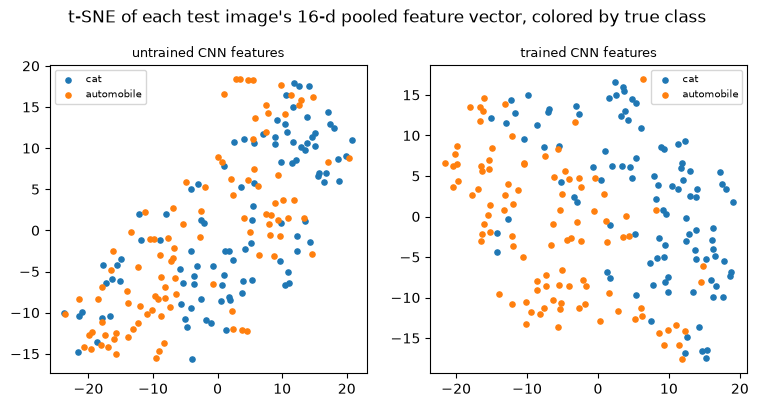
\includegraphics[width=0.9\textwidth]{figures/lesson39_fig03.png}
\caption{t-SNE of each test image's 16-d pooled feature vector, colored by true class: untrained CNN features (left) vs.\ trained CNN features (right).}
\label{fig:l39-3}
\end{figure}

The untrained network's features scatter the two classes together with no visible structure (Figure~\ref{fig:l39-3}) --- unsurprising, since its convolutional weights are still random and have never seen a single labeled example. The trained network's features form two visibly separated clumps, cat and automobile, even though t-SNE itself was never told which point belonged to which class; it only saw the 16-d feature vectors and their pairwise distances. (Quantitatively, a simple 1-nearest-neighbor check in the 2D embedding --- does each point's nearest neighbor share its true label? --- reveals 78\% for the trained features versus about 62\% for the untrained ones.) This is evidence that training didn't just adjust the final linear layer --- it reshaped the whole feature space so that cats and automobiles genuinely live in different neighborhoods of it.

\subsection*{Exercises}
\begin{enumerate}
  \item Grad-CAM here uses the \emph{last} conv layer. Modify \code{grad\_cam} to instead use the intermediate feature map after \code{conv1} (before the pool and \code{conv2}). Does the resulting heatmap get sharper (closer to pixel-perfect, like the saliency map) or coarser, and why would an earlier layer behave that way?
  \item Shrink the marker from $5\times5$ to $2\times2$, or dim it from pure white ($1.0$) to a faint gray ($0.6$). Does \code{model\_shortcut} still learn to rely on it as strongly (check the clean-vs-marked accuracy gap), and does Grad-CAM still catch it as reliably?
  \item The saliency-map gradient in this chapter is taken with respect to the raw logit (\code{score}), not the sigmoid probability. Try computing it with respect to \code{torch.sigmoid(score)} instead --- does the resulting map look meaningfully different, and can you explain why using the chain rule?
  \item Color the trained-feature t-SNE plot by \emph{predicted} label instead of true label. Do the handful of points that land on the ``wrong side'' of the cluster boundary correspond to images the model actually misclassifies? Then repeat with \code{model\_shortcut}'s features on marked vs.\ clean images --- does removing the marker collapse the clean class separation the way the earlier accuracy numbers predicted it would?
\end{enumerate}

\vfill
\fullcode{lesson39}{lesson39_visualizing_cnns}
